\chapter[Materiais e métodos]{Materiais e Métodos}

A análise da viabilidade do sistema foi feita de forma quantitativa por meio de estudo experimental e levantamento de dados em campo, bem como a utilização de software para simulação das reações ocorridas no gaseificador.

	
\section{Aparato experimental}

Para realização dos testes experimentais, foi montado um aparato experimental composto por um reator, um sistema de limpeza dos gases, um grupo moto-gerador e um banco de cargas resistivas para testes no gerador. 

\begin{figure}[!htb]
	\centering
	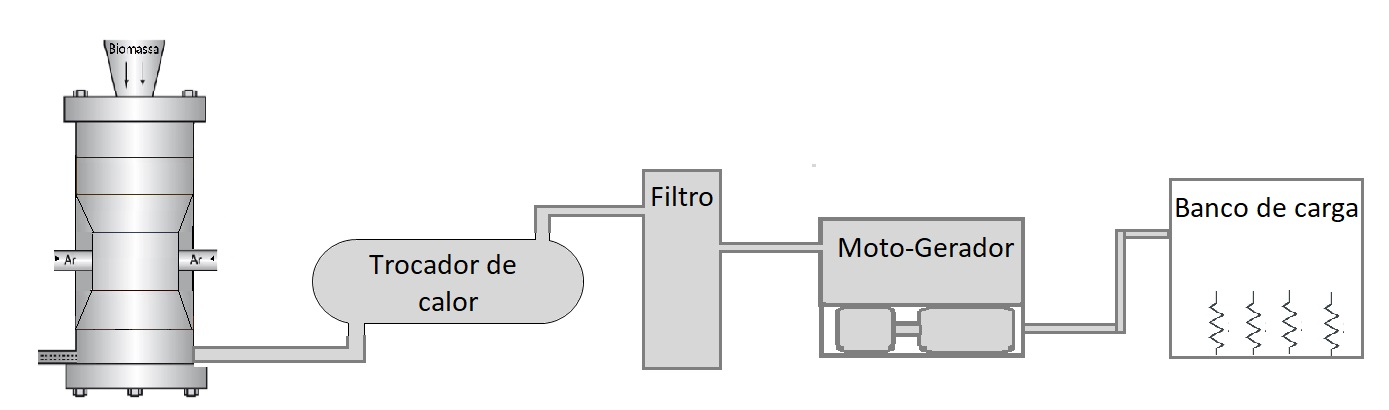
\includegraphics{aparato_experimental}
	\caption{Aparato experimental (Fonte: autoria própria).}
	\label{aparato_experimental}
\end{figure}


O reator utilizado, visto na Figura \ref{foto_reator}, possui 120mm de diâmetro e 480mm de altura.

\begin{figure}[!htb]
	\centering
	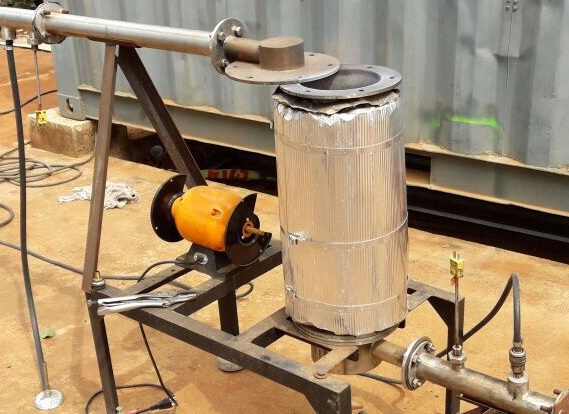
\includegraphics[width=9cm]{gaseificador_foto_3}
	\caption{Reator (Fonte: autoria própria).}
	\label{foto_reator}
\end{figure}

Antes de sua utilização, foram realizadas soldas no seu corpo externo para reparo do material, que tinha fundido. Adicionou-se argamassa refratária na parte interna para evitar transferência de calor com o meio, reduzindo seu diâmetro de 150mm para 120mm. O isolamento térmico foi feito com lã de vidro e manta térmica envoltos por uma cinta térmica.

Para trabahar em modo downdraft, um sistema de admissão de ar e extração de gases foi montado à jusante do reator baseando-se no efeito venturi. Neste sistema, que pode ser visto na Figura *, o ar é puxado por um 

A alimentação da biomassa foi realizada manualmente pelo topo do reator.

O sistema de limpeza foi composto por 

Será utilizado um moto-gerador da Universidade de Brasília - Faculdade Gama movido a gasolina com potência de 1.200W. Uma foto do moto-gerador pode ser vista na Figura \ref{moto_gerador} e suas especificações técnicas podem ser vistas na Tabela \ref{tabela_motor}.

\begin{figure}[!htb]
	\centering
	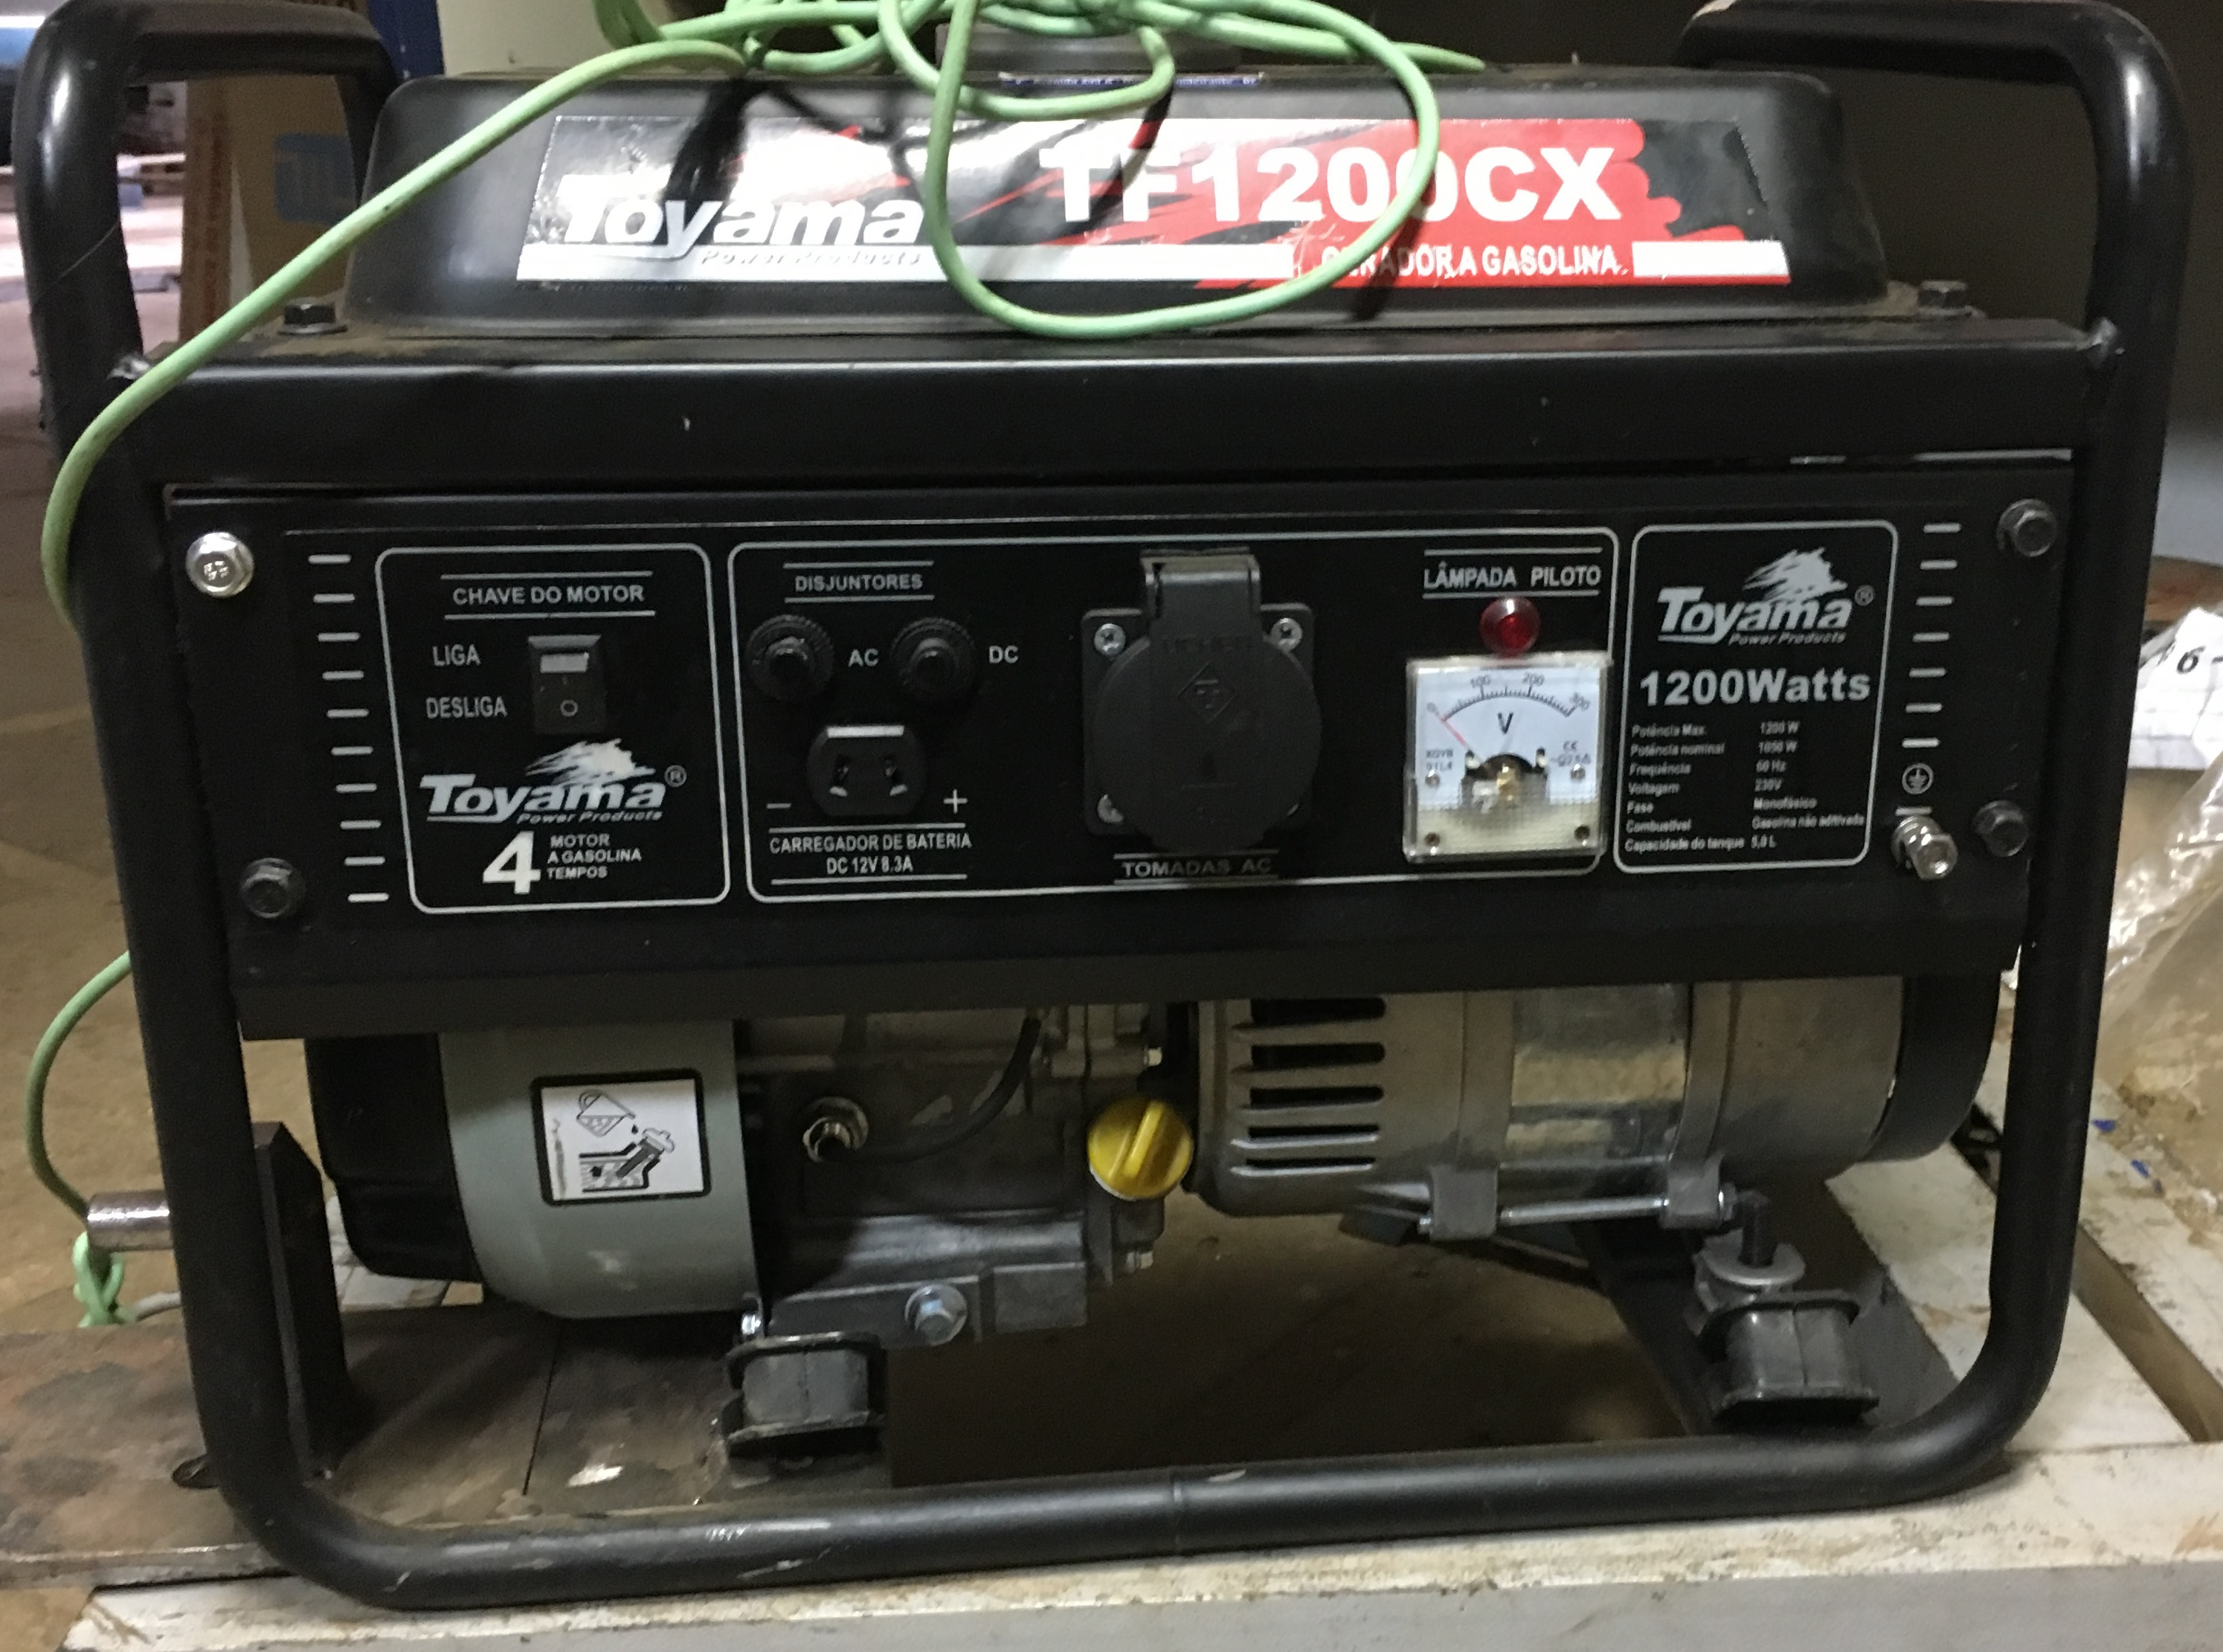
\includegraphics[width=8cm]{moto_gerador}

	\caption{Moto-gerador que será utilizado (Fonte: autoria própria).}
	\label{moto_gerador}
\end{figure}

\begin{table}[h]
	\centering
	\caption{Especificações moto-gerador}
	\begin{tabular}{|l|c|}
		\hline
		\textbf{Marca} & Toyama Power Products \\
		\hline
		\textbf{Potência Máxima} & 1.200 W \\
		\hline
		\textbf{Potência Nominal} & 1.050 W \\
		\hline
		\textbf{Frequência} & 60 Hz \\
		\hline
		\textbf{Voltagem} & 230 V \\
		\hline
		\textbf{Fase} & Monofásico \\
		\hline
		\textbf{Combustível} & Gasolina não aditivada \\
		\hline
		\textbf{Capacidade do tanque} & 5,0 L \\
		\hline
	\end{tabular}
	\label{tabela_motor}
\end{table}	


O banco de carga resistiva foi montado para simular a carga no gerador, além de analisar o consumo de biomassa e o comportamento do sistema quanto a diferentes níveis de carga. O banco foi composto por 


\section{Simulação da reação}

A reação \ref{bagaço_reação} mostra a reação geral de gaseificação do bagaço de cana. Sua fórmula equivalente, C$_x$H$_y$O$_z$N$_w$S$_v$, é obtida através da análise elementar e, como o bagaço de cana é uma biomassa amplamente utilizada e estudada, foi utilizada análise elementar encontrada na literatura.

\begin{equation} \label{bagaço_reação}
C_xH_yO_zN_w + \alpha(O_2 + 3,6N_2) + \beta H_2O \rightarrow aCO_2 + bCO + cH_2 + dO_2 + eH_2 + fCH_4 + gN_2
\end{equation}

A reação \ref{bagaço_reação} e a razão de equivalência serão simulados no software ComGas visando obter um gás de síntese de qualidade com maiores percentuais de CO e H$_2$ e maior poder calorífico.

\subsection{Software ComGas}

O ComGas é um software de simulação de reações de combustão e gaseificação na condição de equilíbrio químico \cite{rendeiro2008}. Sua interface gráfica pode ser vista na Figura \ref{software_comgas}. Nele, é possível introduzir os dados de caracterização do combustível, sendo que alguns fazem parte da base de dados, e a razão de equivalência, bem como determinar se será realizada combustão ou gaseificação, gerando tabelas e gráficos com os resultados de fração molar e mássica dos produtos em função da razão de equivalência, assim como de propriedades do gás como seu poder calorífico.

\begin{figure}[!htb]
	\centering
	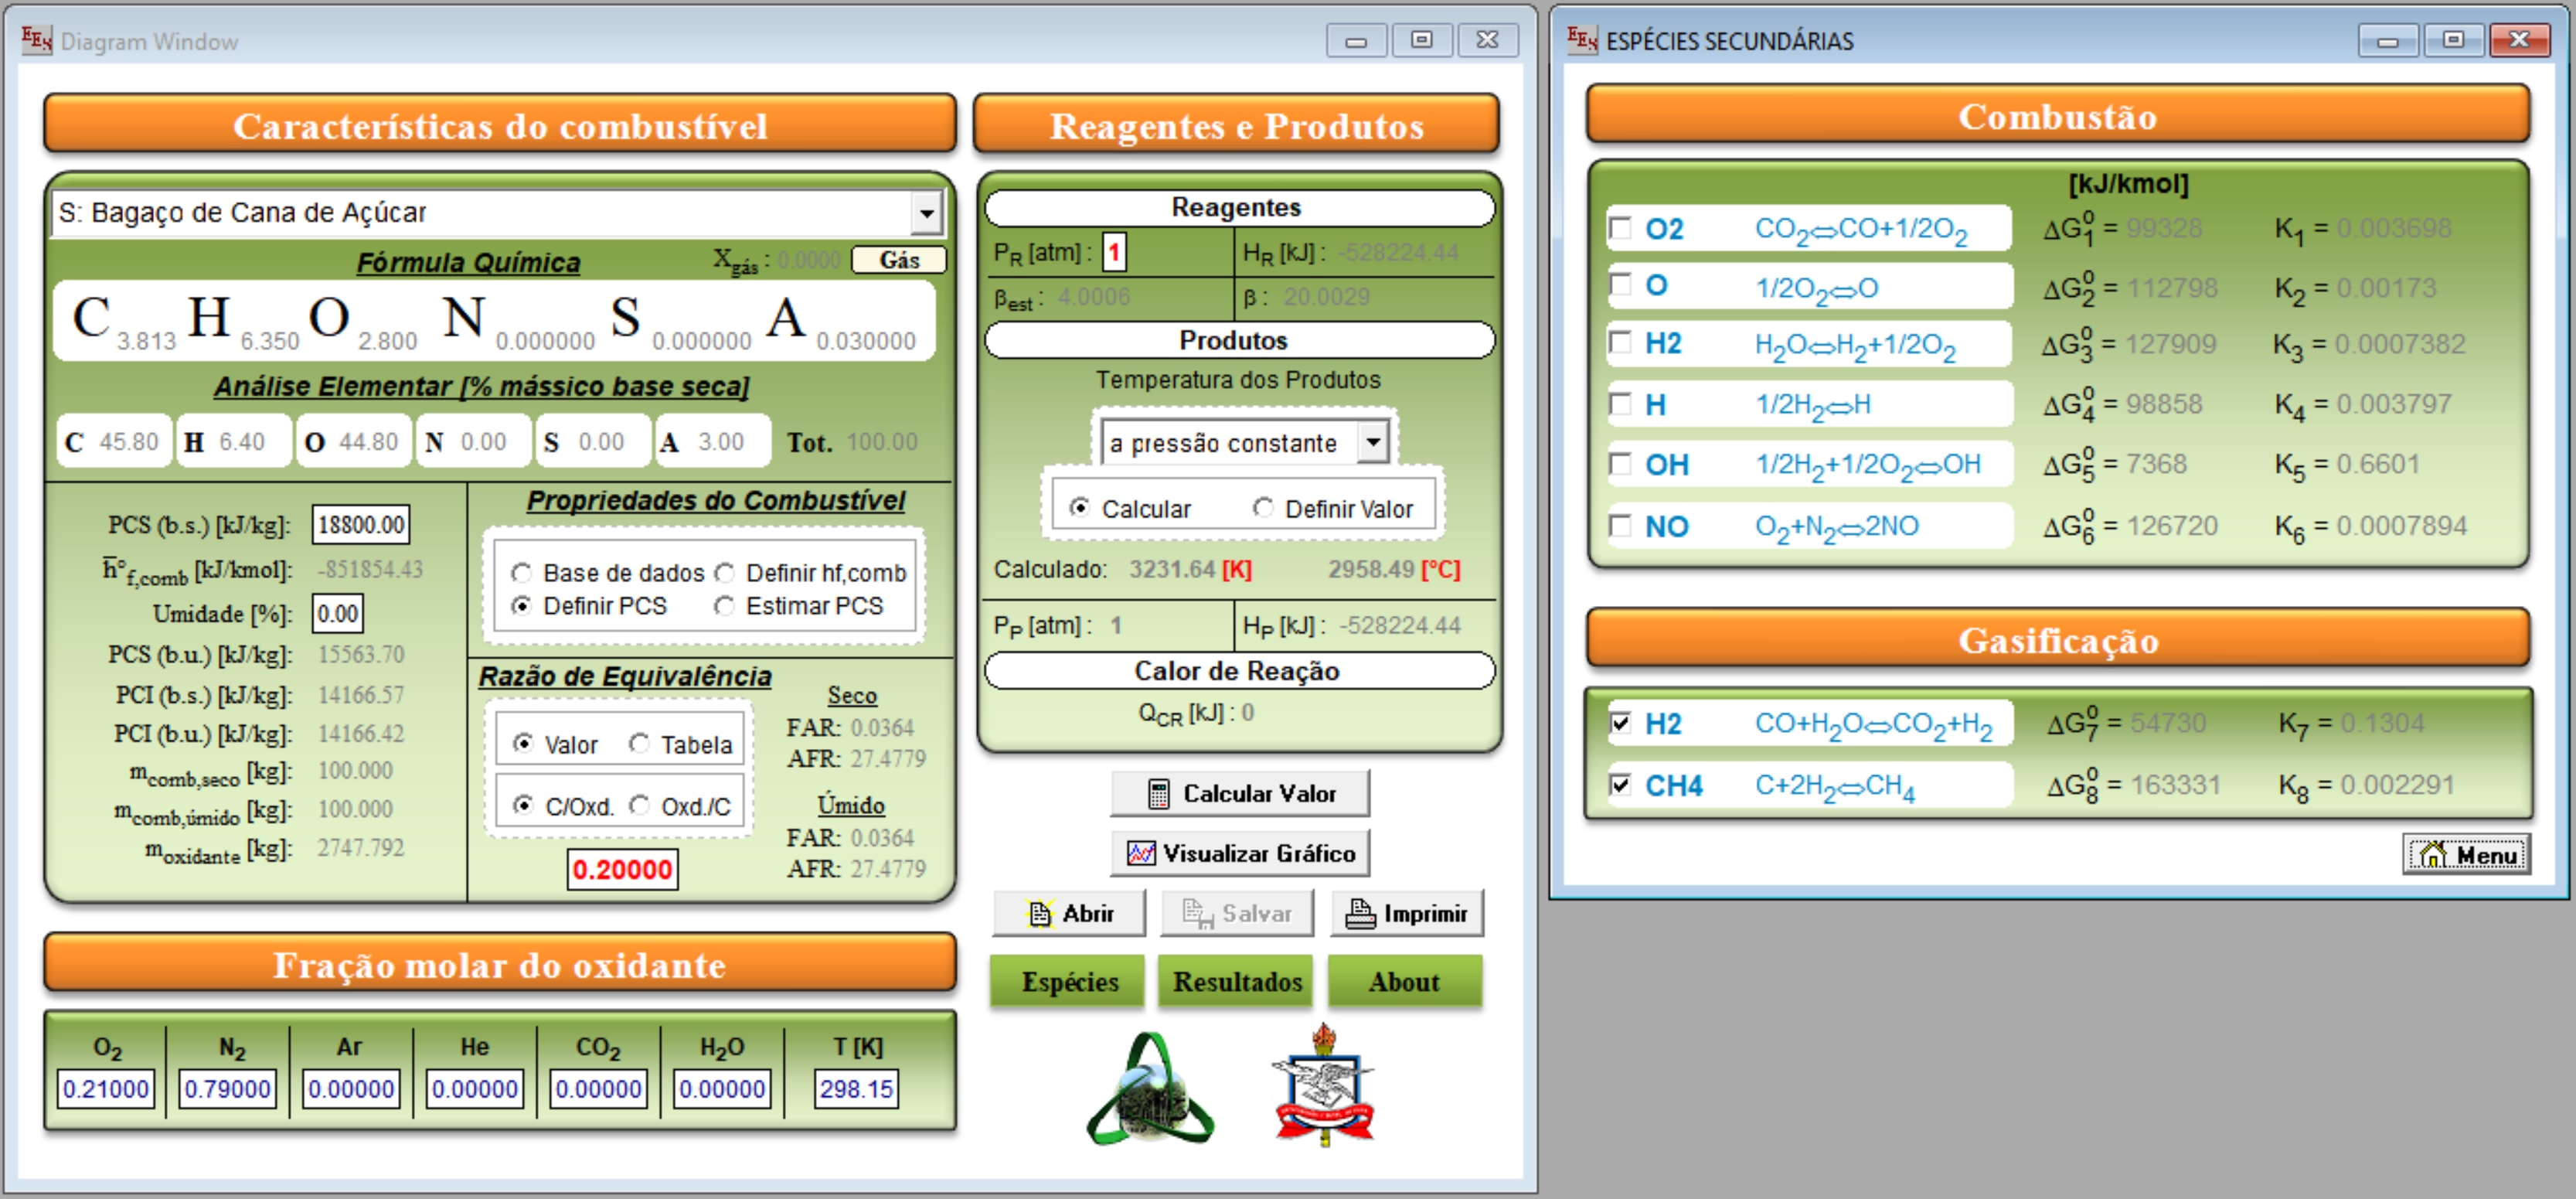
\includegraphics[width = 16cm]{software_comgas}
	\caption{Interface gráfica do software Comgas v1.2 (Fonte:Software Comgas)}
	\label{software_comgas}
\end{figure}

\subsection{Determinação da Vazão de ar}
Para determinar a massa de ar, e assim, a vazão de ar que deve ser inserida no gaseificador, deve-se determinar o valor da razão de equivalência ($\phi$), que é definida como a razão entre a relação ar-combustível (A/C) real e a relação ar-combustível estequiométrico, como mostra a equação \ref{eq:razao_equivalencia}. A relação ar-combustível é dada pela razão entre a massa de ar e a massa de combustível dada na equação \ref{A/C}, onde m\textsubscript{ar} é a massa de ar e m\textsubscript{b} é a massa de bagaço.

Para processos de gaseificação, a razão de equivalência deve ser menor que 1, uma vez que a combustão deve ser incompleta. Geralmente esse valor varia entre 0,2 e 0,4 \cite{narvaez1996}.
 
\begin{equation}\label{eq:razao_equivalencia}
\phi = \frac{A/C\textsubscript{real}}{A/C\textsubscript{estequiométrica}}
\end{equation}
 
\begin{equation}\label{A/C}
A/C = \frac{m\textsubscript{ar}}{m\textsubscript{b}}
\end{equation}


Com o valor das frações molares e mássicas dos produtos obtidos em simulação no software ComGas e calculando a massa de biomassa estequiométrica pela fórmula equivalente, faz-se um balanço de massa da reação, representado na reação \ref{balanço_massa}, onde m\textsubscript{reagentes} é a massa de reagentes e m\textsubscript{produtos} é a massa de produtos, obtendo a massa de ar estequiométrica e, consequentemente, a relação A/C estequiométrica.


\begin{equation}\label{balanço_massa}
m\textsubscript{reagentes} = m\textsubscript{produtos}
\end{equation}

\begin{equation}\label{balanço_ar}
m\textsubscript{b} + m\textsubscript{ar} = m\textsubscript{produtos}
\end{equation}

De posse do valor da razão de equivalência também obtido em simulação, determina-se a relação A/C real. A massa do bagaço de cana será determinada experimentalmente, pesando-a em balança de acordo com o quanto é possível inserir no volume do reator. Calcula-se, então, o volume de ar necessário para gaseificar essa quantidade e o tempo levado para que seja consumida, obtendo a taxa de consumo da biomassa e do ar, podendo, assim, calcular a vazão de ar necessária pela equação \ref{vazao_ar}.

\begin{equation}
A/C\textsubscript{real} = \frac{\dot{m}\textsubscript{ar}}{\dot{m}\textsubscript{b}}
\end{equation}

\begin{equation}\label{vazao_ar}
\dot{v}\textsubscript{ar} = \frac{\dot{m\textsubscript{ar}}}{\rho\textsubscript{ar}}
\end{equation}

\section{Levantamento de dados em campo}

Será realizado levantamento de dados dos equipamentos elétricos com as respectivas potências e da quantidade de bagaço gerada em um pequeno estabelecimento que comercialize caldo de cana para analisar se o bagaço mensal gerado é capaz de produzir a potência máxima do gerador, avaliando a economia que será gerada ao estabelecimento.


